
\label{sec:systemArchitecture}

Dieses Kapitel soll ein Gefühl für die Komponenten von \emph{Flewnit} und 
ihre Zusammenhänge vermitteln. Die Komponenten "`in Aktion"' werden im Detail im Verlauf des Kapitels 
\ref{sec:simulation} beschrieben.

Das System wurde in C++ als (wahlweise statisch oder dynamisch zu linkende) Bibliothek implementiert.
Der Code der GPU-Programme ist in GLSL bzw. OpenCL C verfasst.

\subsection{Dependencies}
	\label{sec:dependencies}
	
	Zunächst sollen die verwendeten Third-Party-Bibliotheken kurz vorgestellt werden:

	\begin{description}
		\item[OpenGL3/4]
		Die schon mehrfach erwähnten modernen Versionen der \linebreak \emph{Open Graphics Library},
		der offenen API der Khronos Group zur \linebreak hardwarebeschleunigten Graphik-Programmierung 
		auf Basis der Dreiecks-Rasterisierung.
		\todo[color=green]{evtl treffenderen Ausdruck finden: Scanline-basiert oder was auch immer}
		Um die Programmierung ohne Legacy-Routinen nicht erst zur Laufzeit über einen OpenCL-Error
		durch Verwendung eines Core-Profiles zu erzwingen, gibt es einen OpenGL- Header
		namens "`gl3.h"'\footnote{beziehbar unter http://www.opengl.org/registry/},
		der in Kombination mit der entsprechenden Präprozessor-Definition
		\lstinline[language=C]|#define GL3_PROTOTYPES 1| schon zur Compile-Zeit nur die non-deprecated
		Routinen zur Verfügung stellt.
		
     	\item[OpenCL 1.0]
	    Die \emph{Open Computing Language}, erste Version der noch jungen API für massiv parallele Programmierung
	    \footnote{die GPGPU-Computing einschließt}, wie OpenGL von der Khronos Group verwaltet; 
	    sie stellt den ersten offenen Standard für GPGPU dar, d.h., die Verwendung der API ist nicht mehr an eine
	    bestimmte Hardware (wie bei Nvidia CUDA) oder ein bestimmtes Betriebssystem (wie Microsofts DirectCompute)
	    gebunden.
	    
	    Zur Zeit der Implementierung waren noch keine Non-Developer-Treiber für OpenCL 1.1 verfügbar, 
	    außerdem gab es kein Feature dieser Version, welches ich dringend benötigt hätte.
	    Deshalb habe ich die Version 1.0 verwendet.
	    
	    Es gibt einen C++ -Wrapper der C-API, welcher stark auf C++-Templates basiert und in einer einzigen Headerdatei 
	    implementiert ist. Dieser ist direkt von der Khronos-Homepage\footnote{http://www.khronos.org/registry/cl/} 	
	    beziehbar. Diesen Wrapper habe ich verwendet, da er die Nutzung der API wesentlich eleganter macht.
	    
    	
   		\item[GLFW 2.7]
		Wie auf Seite \pageref{focus:dependencies} angedeutet, waren mir folgende Dinge wichtig, damit die Einsetzbarkeit
		des Frameworks in professionelleren Kontexten nicht schon im Vorfeld verbaut ist:
		\begin{itemize}
			\item Option auf Fullscreen
			\item Option auf Multisampling
			\item Die Möglichkeit der Erstellung eines OpenGL-Kontextes einer frei wählbaren Version 
			mit Option zwischen Core- und Compatibility-Profile
			\item Option auf "`\emph{Mouse Grab}"', so dass man wie in einem Computerspiel mit ausgeblendetem Mauszeiger
			nur durch Bewegung der Maus ohne Bildschirm-/Fenster-Grenzen die virtuelle Kamera rotieren kann;
			\item "`Input events"', d.h. Aktualisierungen von Benutzereingaben sollen häufig und mit minimaler 
			Latenz geschehen, außerdem so unabhängig wie möglich von der Framerate sein;
			Nach möglichkeit sollten Input-Updates zumindest "aktiv abfragbar" sein 
			(im Gegensatz zum passiven Warten darauf, dass von der Input-Library eine Callback-Funktion 
			aufgerufen wird)
			\item Es soll volle Kontrolle über die "Render-Loop" geben, so dass man nicht 
			den Kontrollfluss an eine Funktion übergibt, die womöglich nie zurückkehrt und weiteren Kontrollfluss
			durch das Benutzerprogramm	nur über Callback-Funktionen ermöglicht
			(wie \lstinline[language=C]|glutEnterMainLoop()| beim in die Jahre gekommenen \emph{GLUT}).
			Ein derartiges Konstrukt ist einer
			Engine nicht würdig und verhindert womöglich sauberes Herunterfahren und Neu-Initialisierung,
			wie es z.B. beim Wechseln einer Szene oder eines fundamentalen globalen Settings nötig sein könnte.	
		\end{itemize}
		\emph{GLFW}\footnote{http://www.glfw.org/} in der Version 2.7, die zum Zeitpunkt der Implementation aktuellste 
		stabile	Version, erfüllt diese Forderungen, und findet damit in \emph{Flewnit} Einsatz sowohl im Fenster- als auch 	
		im Input-Manager. Die Timing-Funktionalität wird ebenfalls von GLFW übernommen.
		
    	
    	\item[GLM]
    	leichte, aber doch recht maechtige mathe-bibliothek
    	
    	\item[Grantlee]
       		die string template engine die CL und GL code erzeugt
       		
    	\item[assimp]
    	

		\item[boost filesystem]
    	
   		\item[TinyXML]
    	- möglichst hohe Konfiguriertbarkeit ohne ständigen recompile: parsing von XML config file
	
	\end{description}	

	
	

    

    	
 

\subsection{Klassendiagramm}

\begin{figure}[!h]
	 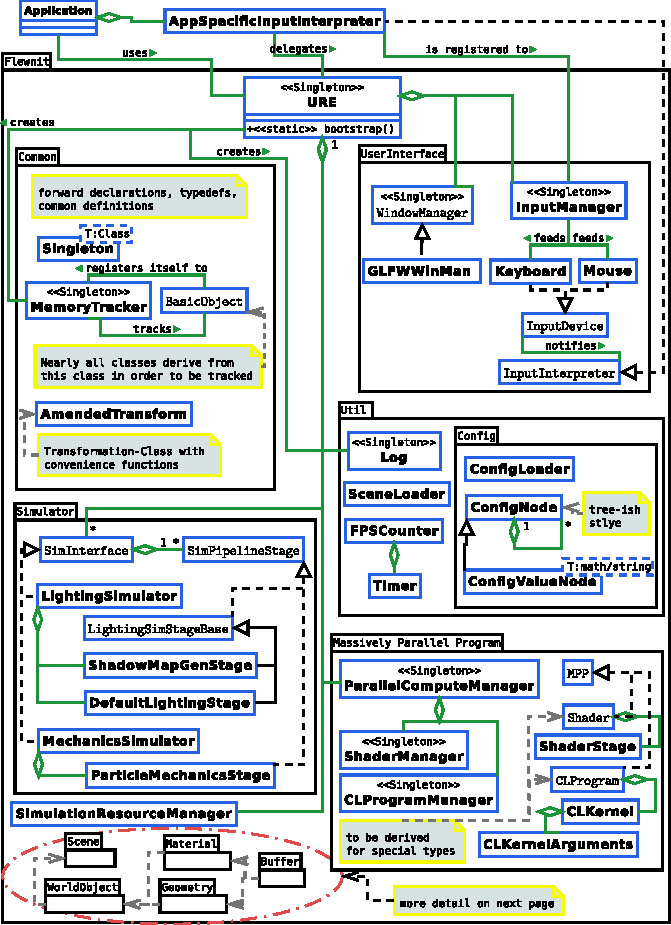
\includegraphics[width=\textwidth]{Overview_Flewnit_Architecture_After_Implementation1.pdf}
	\caption{Klassendiagramm des Gesamtsystems, Teil 1}
	\label{fig:ClassDiagOverview1}
\end{figure}


\begin{figure}[!h]
	 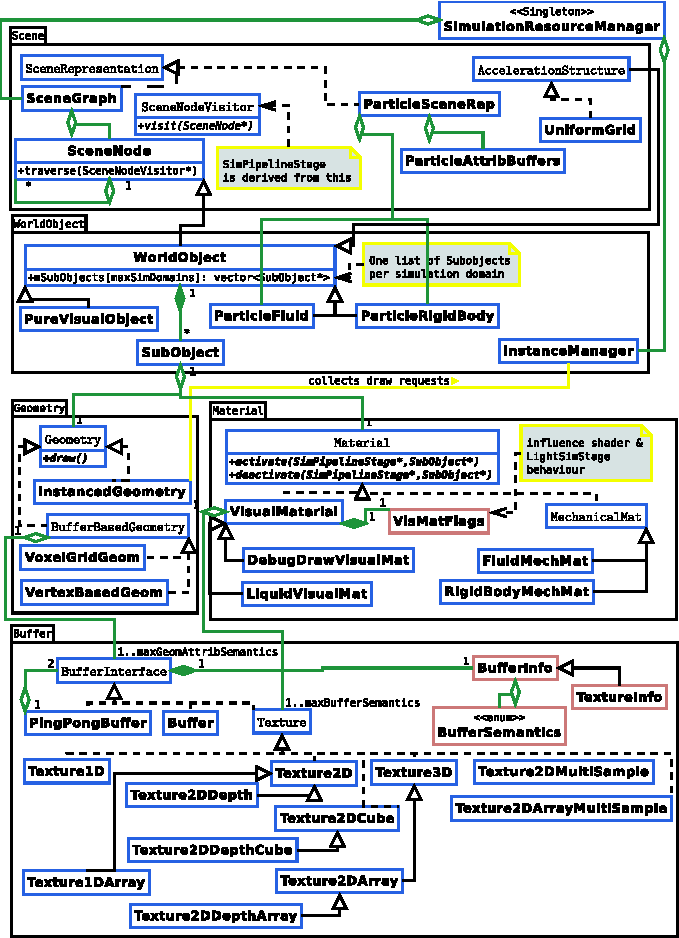
\includegraphics[width=\textwidth]{Overview_Flewnit_Architecture_After_Implementation2.pdf}
	\caption{Klassendiagramm des Gesamtsystems, Teil 2}
	\label{fig:ClassDiagOverview1}
\end{figure}



 
\subsection{BasicObject und Memory Tracking}
	 für vielseitig, flexible anwendung zur Laufzeit sollten keine 	Speicher-Lecks auftreten damit Funktionalität 
	 kontrolliert heruntergefahren und neu initialisiert werden kann; 
	 	- memory tracking, (erklären, warum nicht tracking mit Valgrind)
 
    	
\subsection{Die \emph{Unified Rendering Engine}}
URE blubb

\subsection{Die Simulator-Klassen}


\subsection{Die SimulationPipelineStages}
	shdow map gen, direct lighting, rendering features particlemechanics stage;
	in planung: deferred rendering G-Bufferfill, deferred rendering shade, div. post processing stages


\subsection{Die Manager-Klassen}
Für gemeinsamen zugriff sollten viele Daten für andere Klassen verfügbar sein (Buffer, Rendering Results...); 	
Realisierung über Manager-Singleton-Klassen und Zugriff über Map-Container;
\todo[color=green]{evtl. andere reihenfolge}

\subsection{Die Template-Engine}
	\label{sec:architecture:templateEngine}
	exemplarischer code schnipsel, refernz su shadermanager und CLProgramManager, erklärung wie man templat contex setzt, 	
	vererbung etc;
    	
\subsection{Die Buffer-Abstraktion}  
	\label{sec:architecture:BufferAbstraction} 	
 	die bombe, die cpu, ogl und ocl vereint, inclusive ping ponging etc.. 
 	fundamentale Klassensammlung fuer den Unified-Aspekt
 	
 	\begin{figure}[!h]
  		\begin{tabular}
  		{
  		 l  l | c | c | c |
  		}
																	\cline{3-5}
  									&								&	\multicolumn{3}{ c | }{Context} \\ 
  																	\cline{3-5}
									&								& 	Host 	& 	OpenGL 	& 	OpenCL	\\
    	\noalign{\hrule}								
    	\multicolumn{1}{|c|}{
    		generic Buffer
    	}							& 								
    		&	{\color{green}\checkmark} 	&	{\color{red}x}		& 	{\color{green}\checkmark}	\\ 
    	
    	\noalign{\hrule}								
    	\multicolumn{1}{|c|}{
    		\multirow{4}{*}{OpenGL Buffers}
    	}							& Vertex Attribute Buffer		
    		&	{\color{orange}o} 	&	{\color{green}\checkmark}		& 	{\color{orange}o}	\\  
    								\cline{3-5}
    	\multicolumn{1}{|c|}{}		& Vertex Index Buffer			
    		&	{\color{orange}o} 	&	{\color{green}\checkmark}		& 	{\color{orange}o}	\\  
    								\cline{3-5}
    	\multicolumn{1}{|c|}{}		& Uniform Buffer
    		&	{\color{orange}o} 	&	{\color{green}\checkmark}		& 	{\color{orange}o}	\\ 
    								\cline{3-5} 
    	\multicolumn{1}{|c|}{}		& Render Buffer					
    		&	{\color{red}x} 	&	{\color{green}\checkmark}		& 	{\color{green}\checkmark}	\\ 
    
   		\noalign{\hrule}								
   		\multicolumn{1}{|c|}{
    		\multirow{4}{*}{Textures} 
   		}							& 1D Texture					
   			&	{\color{orange}o} 	&	{\color{green}\checkmark}		& 	{\color{red}x}	\\ 
    								\cline{3-5}
		\multicolumn{1}{|c|}{}		& 2D Texture				
			&	{\color{orange}o} 	&	{\color{green}\checkmark}		& 	{\color{green}\checkmark}	\\ 
									\cline{3-5}
		\multicolumn{1}{|c|}{}		& 3D Texture		
			&	{\color{orange}o} 	&	{\color{green}\checkmark}		& 	{\color{green}\checkmark}	\\ 
									\cline{3-5}
		\multicolumn{1}{|c|}{}		& Special Texture				
			&	{\color{orange}?} 	&	{\color{green}\checkmark}		& 	{\color{orange}?}	\\ 


    	\noalign{\hrule}
     
     	
  		\end{tabular}	
  	
  		\caption{		
  			Verschiedene Buffertypen und ihre Verfügbarkeit in verschiedenen Kontexten \\	
  			Legende: \\
			{\color{green}\checkmark}	$\rightarrow$ nativ unterstützt;
			{\color{orange}o}	$\rightarrow$ kompatibel;
			{\color{red}x}	$\rightarrow$ nicht unterstützt;	\\
			{\color{orange}?}	$\rightarrow$ Unterstützung abhängig von weiteren Parametern;	
		}
	
  	\end{figure}
 
\subsection{Das WorldObject}
	Basis-Klasse fuer alles was unified simuliert wird: pure viuelle objekt, uniform grid, fluid, rigid body etc..
	
	\subsubsection{Das SubObject}
  
 
\subsection{Material}  
	was stellt welches material in welcher Domain dar?
	
\subsection{Geometry}
	Abtract, Buffer based, Vertex based etc.. ein paar konzepte (implementiert/genutzt nur VertexBased)  
	
\subsection{Massively Parallel Program}
	Basisklasse von Shader und OpenCL Program
	\subsubsection{Shader}
		
	\subsubsection{OpenCLProgram}

weitere klassen/konzepte to go...	


\subsection{Status der Implementierung am Ende der BA}
	
	Features auflisten;
	\todo[color=green]{screenshots? oder lieber erst später,zusammen mit detaillierter erläuterung?}

	großteils programmierte, aber ungenutzte/ungetestete features erwähnen (Deferred Rendering, Layered Rendering, 	
	RenderTarget-Klasse, Partikel-Rigid bodies, verschiedene Fluid-Typen); 


	überlegte aber nciht programmierte Konzepte/Algorithmen erwähnen (Triangle-Index-Voxelisierung)
	
	schlimmste schnitzer nennen, wie
		- miese fluid-visualisierung, 
		- unübersichtliche shadertemplates, besser gemacht bei CL-
			Kernel-Templates, 1. weil struktur hier besser "vererbbar", 2. weil mehr erfahrung mit  Template-Engine
	
	  	
  	

\clearpage
